\chapter{Methodology}
This chapter serves as the blueprint for the empirical study conducted in this thesis. It outlines the critical components of the research, including datasets, ranking models, training procedures, query generators, and evaluation metrics. Additionally, the preparatory steps taken to set up the experimentation environment are outlined. This chapter offers transparency into the experimental framework and how the research questions will be addressed by delineating the methodology employed. It lays the groundwork for comprehending the subsequent results and their implications.

\begin{figure}[h]
\centering
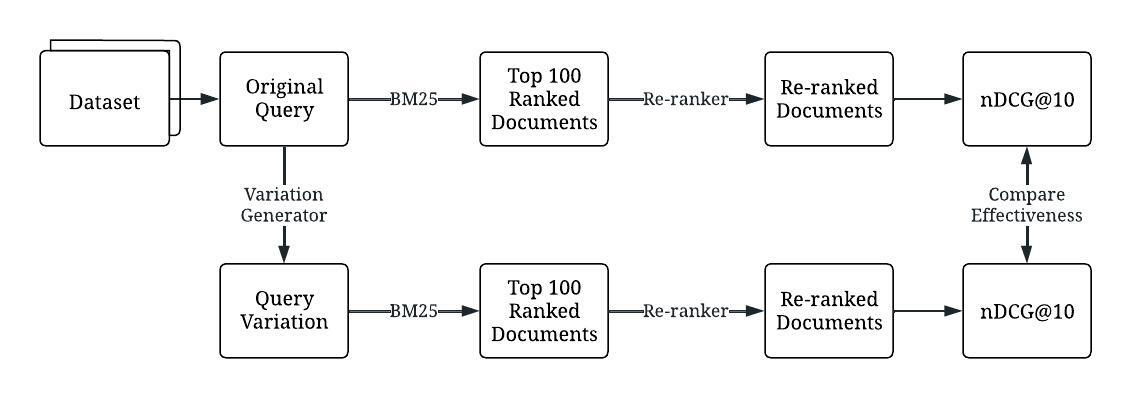
\includegraphics[width=\textwidth]{4Methodology/method.jpeg}
\caption{Flowchart illustrating the methodology workflow.}
\label{fig:method}
\end{figure}

\section{Datasets}
The original study leverages two distinct datasets to investigate the reproducibility and expansion of prior findings.

The first dataset, TREC-DL-2019 \cite{trec}, is a benchmark for passage retrieval tasks and comprises a test set featuring 43 diverse queries. These queries serve as the basis for exploring the impact of query variations on retrieval pipelines. The dataset was selected for its diversity and established use in retrieval research.

The second dataset, ANTIQUE \cite{antique}, focuses on non-factoid question answering and includes a test set with 200 distinct queries. These queries provide additional depth to the research by covering a broader range of information retrieval scenarios.

Incorporating both the datasets from the original study and introducing new ones for expansion was a reasonable approach to ensure the thoroughness and generalisability of the research findings. Using the datasets from the original study provided continuity and allowed for the replication of experimental conditions. This ensures that the reproducibility aspect of the research question can be rigorously examined, as any variations in results can be attributed to the models and methodologies rather than differences in datasets.

On the other hand, introducing new datasets broadened the scope of the study and extended its applicability to a broader range of information retrieval scenarios. This expansion allows for exploring how the conclusions and observations drawn from the original datasets generalise to different contexts and data characteristics. By combining existing and novel datasets, the research balances between validating previous findings and advancing our understanding of query variation impacts on retrieval pipelines in diverse settings.

\subsection{DL-TYPO Dataset}
The DL-TYPO dataset, introduced by Zuccon and Zhuang, stands as a valuable resource for scrutinizing the resilience of retrieval systems when confronted with real-world query variations, specifically those encompassing typographical errors. Within this dataset, one finds a collection of human relevance judgments and query pairs, each set consisting of queries with typos and their corrected counterparts. A distinctive hallmark of the DL-TYPO dataset lies in its unique origin: queries are sourced directly from a sizeable search engine query log, thus presenting genuine depictions of real-world queries and the inherent typographical mistakes that naturally arise.

Table 1 provides illustrative examples of original queries extracted from this dataset, juxtaposed with their corrected versions, showcasing various typographical error types, such as extra characters, missing characters, character transpositions, or the use of incorrect characters. These errors closely mirror the typographical variation techniques employed in the original study.

The deliberate choice to employ the DL-TYPO dataset with misspellings, despite the availability of a version free from such errors, was driven by several key considerations. Foremost, the version without misspellings was expected to yield results akin to those derived from the TREC-DL-2019 dataset. A misspelling-free dataset in this context would have added little novelty or experimental diversity.

The primary rationale for opting for the version inclusive of misspellings lies in pursuing a novel perspective on retrieval system behaviour in the presence of real-world query variations. By introducing queries with genuine typographical errors, researchers aimed to evaluate how retrieval systems adapted and performed under more challenging conditions. This presented an element of unpredictability and complexity, reflecting that real-world users often introduce typos or variations into their queries, necessitating retrieval systems to exhibit robustness in handling such scenarios effectively.

Furthermore, researchers were eager to assess the impact of typo variation generators when operating alongside misspellings. These generators constitute a critical component in studying retrieval systems, simulating the creation of queries with various forms of variation, including typos and using the DL-TYPO dataset with misspellings allowed researchers to explore how these generators interacted with authentic misspellings present in the dataset. This approach not only enriched the understanding of typo generation but also yielded insights into the retrieval system's ability to handle such generated variations effectively.

\begin{table}[h]
\centering
\caption{Examples of original queries and their corrected counterparts from DL-TYPO illustrating various misspelling errors. The spelling error is bolded.}
\label{tab:dl-egs}
\begin{tabularx}{\columnwidth}{X|X|X}
\textbf{Original Query} & \textbf{Corrected Query} & \textbf{Misspelling Type} \\ \hline
\textbf{a}red hat society & red hat society & Extra character \\
cache creek casi\textbf{on} & cache creek casi\textbf{no} & Neighbouring character swap \\
car accident lawers & car accident law\textbf{y}ers & Missing character \\
how to clear bad e\textbf{x}zema & how to clear bad e\textbf{c}zema & Incorrect character \\ \hline
\end{tabularx}
\end{table}
Additionally, relevance assessments are provided against passages from the MSMARCO dataset, an established resource for information retrieval research. Investigating the performance of retrieval models on this dataset allows for meaningful conclusions to be drawn about the effectiveness and robustness of such models in handling actual typos. Moreover, the statistical analysis and benchmarking conducted on this dataset, using standard evaluation metrics, provide a solid foundation for comparative research. 

In summary, the decision to employ the DL-TYPO dataset with misspellings was motivated by the quest to introduce a fresh perspective into the research, challenge retrieval systems with real-world query variations, and investigate the interaction between typo variation generators and authentic misspellings, ultimately enhancing the depth and comprehensiveness of the research findings. The dataset topics and qrels were sourced from \url{https://github.com/ielab/CharacterBERT-DR}.

\section{Ranking Models and Training}
The selection of models in the original study was driven by the need to comprehensively assess the robustness of retrieval pipelines when exposed to query variations. To achieve this goal, a diverse range of ranking models was chosen to represent different paradigms and approaches within the field of information retrieval.

As depicted in Figure \ref{fig:method}, the retrieval process involves the initial application of BM25 as a first-stage retrieval method. Subsequently, the top 100 retrieved results undergo a re-ranking process using one of the following models: RM3, KNRM, CKNRM, EPIC, BERT, or T5. The resulting re-ranked documents are then employed to assess retrieval effectiveness. This comprehensive evaluation procedure is conducted for each original query and its corresponding query variations within the three datasets.

\begin{itemize}
    \item Traditional Models (Trad): BM25 \cite{bm25} and RM3 \cite{rm3} utilised default hyperparameters and the implementation provided by the PyTerrier toolkit \cite{pyterrier}.
    \item Neural Ranking Models (NN): Kernel-based ranking models KNRM \cite{knrm}, and CKNRM \cite{cknrm} were trained on the training sets of TREC-DL-2019 and ANTIQUE, employing default settings from the OpenNIR \cite{opennir} implementation.
    \item Transformer-Based Models (TNN): BERT-based methods, including EPIC \cite{epic} and BERT \cite{bert}, underwent fine-tuning using the bert-base-uncased model on the respective training datasets. T5 \cite{t5} models were implemented using the monoT5 \cite{monot5} framework from the PyTerrier T5 plugin, incorporating pre-trained weights for MSMarco \cite{msmarco} by the original authors of monoT5.
\end{itemize}

Using the same models from the original study without introducing any new ones was a deliberate choice to ensure the research's reproducibility and comparability. By maintaining consistency with the models used in the original study, this thesis focused primarily on reproducing the findings and expanding upon them through additional datasets, thus allowing for a more direct evaluation of the study's original observations. Furthermore, the original study had already carefully selected a diverse set of ranking models that represented various paradigms within information retrieval, making them well-suited for a reproducibility study and the subsequent expansion. This approach ensures that any differences or improvements observed in the new datasets can be more confidently attributed to variations in query generation and the nature of the datasets rather than introducing new ranking models. It also facilitates a direct comparison of the results with those of the original study, enabling a comprehensive assessment of the generalisability of the findings across different contexts.

\section{Query Variations}
\subsection{Taxonomy}
In the original study, the investigation of query variations was centred around utilising the UQV100 \cite{uqv} dataset. The dataset, curated for this purpose, encompasses query variations for 100 subtopics drawn from the TREC 2013 and 2014 web tracks. This dataset is quite substantial, containing 365,000 query variation pairs. From this vast collection, the study randomly selected 100 pairs for manual annotation and in-depth analysis.

During the annotation process, the authors meticulously categorised these query pairs into six transformation categories. The aim was to differentiate between variations that altered the semantics of the query and those that preserved its original meaning. These categories provided a structured framework for understanding the nature of query variations and their potential impact. The original study, illustrated by Table \ref{tab:var-types}, introduced and elaborated on these six categories, offering clear definitions and representative examples extracted from the UQV100 dataset.

\begin{table}[h]
\centering
\caption{Query Variation Taxonomy with examples from UQV100 Dataset.}
\label{tab:var-types}
\resizebox{\columnwidth}{!}{%
\begin{tabular}{l|l|l|lcl}
\begin{tabular}[c]{@{}l@{}}\textbf{Changes}\\ \textbf{semantics}\end{tabular} & \textbf{Category} & \textbf{Definition} & \multicolumn{3}{l}{\textbf{Examples from UQV100}} \\ \hline
\multirow{2}{*}{Yes} & Gen./specialization & \begin{tabular}[c]{@{}l@{}}Generalizes or special-\\izes within the same\\information need.\end{tabular} & \multicolumn{1}{l}{\begin{tabular}[c]{@{}l@{}}american civil\\war\end{tabular}} & \multicolumn{1}{c}{$ \leftrightarrow $} & \begin{tabular}[c]{@{}l@{}}number of battles\\in south carolina\\during civil war\end{tabular} \\ \cline{2-6} 
 & Aspect Change & \begin{tabular}[c]{@{}l@{}}Moves between related\\but different aspects\\within the same infor-\\mation need.\end{tabular} & \multicolumn{1}{l}{\begin{tabular}[c]{@{}l@{}}what types of spi-\\ders can bite you\\while gardening\end{tabular}} & \multicolumn{1}{c}{$ \leftrightarrow $} & {\begin{tabular}[c]{@{}l@{}}signs of spider\\bite\end{tabular}} \\ \hline
\multirow{4}{*}{No} & Misspelling & \begin{tabular}[c]{@{}l@{}}Adds or removes spell-\\ing errors.\end{tabular} & \multicolumn{1}{l}{raspberry pi} & \multicolumn{1}{c}{$ \leftrightarrow $} & raspeberry pi \\ \cline{2-6} 
 & Naturality & \begin{tabular}[c]{@{}l@{}}Moves between keyword\\and natural language\\queries.\end{tabular} & \multicolumn{1}{l}{\begin{tabular}[c]{@{}l@{}}how does zinc\\relate to wilson’s\\disease\end{tabular}} & \multicolumn{1}{c}{$ \leftrightarrow $} &{\begin{tabular}[c]{@{}l@{}} zinc wilson’s\\disease\end{tabular}} \\ \cline{2-6} 
 & Ordering & \begin{tabular}[c]{@{}l@{}}Changes the order of\\words.\end{tabular} & \multicolumn{1}{l}{\begin{tabular}[c]{@{}l@{}}carotid cavernous\\ fistula treatment\end{tabular}} & \multicolumn{1}{c}{$ \leftrightarrow $} & \begin{tabular}[c]{@{}l@{}}treatment carotid\\ cavernous fistula\end{tabular} \\ \cline{2-6} 
 & Paraphrasing & \begin{tabular}[c]{@{}l@{}}Rephrases the query by\\modifying one or more\\words.\end{tabular} & \multicolumn{1}{l}{\begin{tabular}[c]{@{}l@{}}cures for a bald\\spot\end{tabular}} & \multicolumn{1}{c}{$ \leftrightarrow $} & cures for baldness \\ \hline
\end{tabular}%
}
\end{table}

Furthermore, an additional set of 550 query variation pairs was labelled to gauge the distribution of these categories, and inter-annotator agreement was found to be moderate. The study's findings revealed that most query variations (57\%) pertained to changes in query syntax without altering the query's underlying semantics. This significant discovery led the research to focus primarily on syntax-changing query variations, deferring the exploration of other categories for future research.

\subsection{Variation Generators}
To explore the generation of query variations within the syntax-changing categories, this study employed a multi-faceted approach. Initial investigations included exploring different query generation techniques tailored to each category, followed by a meticulous filtering process. The filtering was designed to select only those methods capable of producing valid query variations while simultaneously eliminating approaches that exhibited high correlations with each other.

\begin{table}
\caption{Outline of each of the ten variation generator methods used.}
\resizebox{\columnwidth}{!}{%
\label{tab:var-gens}
\begin{tabular}{l|l|l}
\textbf{Category} &
  \textbf{Method} &
  \textbf{Definition} \\ \hline
\multirow{3}{*}{Misspelling} &
  NeighbCharSwap &
  \begin{tabular}[c]{@{}l@{}}Swaps two neighbouring characters from a random\\query term (excluding stopwords).\end{tabular} \\ \cline{2-3} 
 &
  RandomCharSub &
  \begin{tabular}[c]{@{}l@{}}Replaces a random character from a random query\\term (excluding stopwords) with a randomly\\chosen new ASCII character.\end{tabular} \\ \cline{2-3} 
 &
  QWERTYCharSub &
  \begin{tabular}[c]{@{}l@{}}Replaces a random character of a random query\\term (excluding stopwords) with another character\\from the QWERTY keyboard, mimicking typing\\errors.\end{tabular} \\ \hline
\multirow{2}{*}{Naturality} &
  RemoveStopWords &
  \begin{tabular}[c]{@{}l@{}}Removes all stopwords from the query, transform-\\ing natural language queries into keyword queries. \end{tabular}\\ \cline{2-3} 
 &
  T5DescToTitle &
  \begin{tabular}[c]{@{}l@{}}Applies an encoder-decoder transformer model (T5)\\fine-tuned to generate the title of a TREC topic\\title based on the topic description.\end{tabular} \\ \hline
Ordering &
  RandomOrderSwap &
  \begin{tabular}[c]{@{}l@{}}Randomly swaps two words of the query, shuffling\\word order.\end{tabular} \\ \hline
\multirow{4}{*}{Paraphrasing} &
  BackTranslation &
  \begin{tabular}[c]{@{}l@{}}Applies a translation method to the query, trans-\\lating it to a pivot language and back to the orig-\\inal language, generating paraphrases.\end{tabular} \\ \cline{2-3} 
 &
  T5QQ &
  \begin{tabular}[c]{@{}l@{}}Utilises an encoder-decoder transformer model (T5)\\fine-tuned to generate a paraphrase question from\\the original question \cite{desctitle}.\end{tabular} \\ \cline{2-3} 
 &
  WordEmbedSynSwap &
  \begin{tabular}[c]{@{}l@{}}Replaces a non-stop word by a synonym based on\\the nearest neighbour word in the embedding\\space, using counter-fitted Glove embeddings \cite{glovefit}.\end{tabular} \\ \cline{2-3} 
 &
  WordNetSynSwap &
  \begin{tabular}[c]{@{}l@{}}Replaces a non-stop word by the first synonym\\found on WordNet (https://wordnet.princeton.edu/);\\if no valid synonyms are available, it does not output\\a valid variation.\end{tabular} \\ \hline
\end{tabular}%
}
\end{table}
Ultimately, the research identified and utilised ten distinct query variation generation methods, each enumerated in Table \ref{tab:var-gens}. Additionally, the table provides an illustrative example of the transformation performed by each method when applied to an input query. It's worth noting that while most of these methods have the potential to generate multiple variations for a single input query, the study chose to present a single query variation per method, thereby ensuring a rich and diverse dataset for subsequent analysis.

For instance, in the case of T5DescToTitle and T5QQP, pre-trained T5 models (specifically, t5-base) were fine-tuned using the Huggingface transformers library \cite{hugging}. On the other hand, the facebook/m2m100\_418M pre-trained model, available through the transformers library, and the M2M100 model \cite{translation} were employed for the BackTranslation method. All other query variation methods relied on the TextAttack library implementation \cite{textattack}, underlining the diverse set of tools and techniques used to generate query variations for this study.

\section{Evaluation Metrics}
In this section, we elaborate on the choice of evaluation metric and the rationale behind exclusively employing nDCG@10 (normalised Discounted Cumulative Gain at rank 10) as the primary metric in this study. The decision to use nDCG was rooted in its suitability for information retrieval tasks, especially when ranking results are paramount. This metric served as a means to assess the effectiveness of ranking models in retrieving relevant documents.

The exclusive reliance on nDCG as the sole evaluation metric in the thesis was a conscious and well-founded decision driven by several compelling reasons. To begin with, nDCG enjoys widespread recognition and acceptance within the field of information retrieval. This made it not only suitable for comparing our results with existing research but also ensured consistency in the evaluation process across different studies.

Furthermore, nDCG's intrinsic ability to consider document relevance and ranking position provides a comprehensive and holistic assessment of the retrieval pipeline's performance. This alignment with the research objectives was crucial as it enabled us to evaluate the impact of query variations on the quality of ranked results comprehensively. Introducing additional metrics could have complicated the analysis and potentially led to conflicting results, making it challenging to draw clear and meaningful conclusions.

Finally, our exclusive focus on nDCG allowed us to delve deeper into the nuances and specific effects of query variations on the performance of the retrieval pipeline. This, in turn, provided us with a comprehensive understanding of the research questions. In essence, the decision to rely solely on nDCG was made to maintain methodological rigour, ensure that our results were meaningful and interpretable, and facilitate a focused investigation into the reproducibility and generalisability of the original study's findings while keeping the research methodology clear and straightforward.

\section{Environment Setup and Pre-Experimentation Steps}
Before delving into the experimentation phase of the project, a series of critical steps were undertaken to ensure the setup and readiness of the environment. This section outlines the decisions and actions to create a conducive experiment environment.

\subsubsection{Exploration of Environment Options}
Initially, the project considered several avenues for setting up the experimentation environment. These options included running experiments on a personal laptop and utilizing the Rangpur cluster. However, both of these approaches encountered limitations that hindered progress. The personal laptop lacked a GPU, which is essential for resource-intensive experiments, and the Rangpur cluster did not have the required version of Python, which posed compatibility challenges.

\subsubsection{Adoption of Google Colab}
After carefully evaluating the available options, it was decided that conducting all experiments via a Google Colab notebook would be the most practical and effective approach. Google Colab provided several advantages, including a straightforward and organised environment for experimentation and the availability of GPU resources. To ensure seamless access to the necessary computational power, a Colab Pro subscription was purchased for the project's duration.

To facilitate experimentation, a new Google Colab notebook was created based on the original project repository. This notebook was then adapted to serve as the central hub for cloning the original repository, the CharacterBERT repository, and executing all the essential experimental steps.

\subsubsection{Pre-Experimentation Setup}
Before conducting the experiments, several preparatory steps were executed, including but not limited to:

\begin{itemize}
    \item Environment Configuration: The notebook was configured to ensure all required libraries and dependencies were correctly installed and configured for the project's needs.
    \item Indexing Documents: A vital modification was made to address issues related to document indexing, which had been broken in the original codebase. This adjustment was crucial for ensuring the accurate retrieval of relevant documents during experiments.
    \item Codebase Enhancements: Changes and additions were made to enhance the codebase, including improving code cleanliness, updating scripts for running reproduction steps, and adapting query rewriting and rank fusion methods to accommodate datasets not sourced from the standard ir\_datasets repository.
\end{itemize}

By systematically addressing these pre-experimentation steps, the project established a robust foundation for conducting experiments, ensuring that the environment was configured correctly and that the necessary data and tools were readily available for the forthcoming research phases.
